\documentclass{article}
\usepackage[]{graphicx}
\usepackage[]{unicode-math}
\usepackage[utf8]{inputenc}
\usepackage[]{booktabs}
\usepackage{nicematrix}

\NiceMatrixOptions{
code-for-first-row = \color{blue} ,
code-for-last-row = \color{blue} ,
code-for-first-col = \color{blue} ,
code-for-last-col = \color{blue}
}

\title{UNLP-Stars: A Large Dataset for the detection of Be and EM stars using Machine Learning}



\begin{document}

\maketitle

\section{Q-Features}

$Q$ Features provide a way to remove the effect of distances and reddening on magnitudes.


Given input magnitudes $m_i$ $i=1,\dots,M$ and corresponding magnitude coefficients $c_i$, we define $q^3$ and $q^4$ features as:
$$
\begin{aligned}
    c^3_{i,j,k} &= \frac{c_i-c_j}{c_j-c_k}\\
    q^3_{i,j,k} &= m_i - m_j - c^3_{i,j,k} (m_j-m_k)     
\end{aligned}
$$

$$
\begin{aligned}
    c^4_{i,j,k,l} &= \frac{c_i-c_j}{c_k-c_l} \\
    q^4_{i,j,k,l} &= m_i - m_j - c^4_{i,j,k,l} (m_k-m_l)     
\end{aligned}
$$

$Q$ features are defined over the set of all possible 3 and 4 sized permutations of the magnitudes, since interchanging indexes $i,j,k$ or $i,j,k,l$ can yield different $q$ values with appropriate $c_i$ coefficients. The generation of all possible $Q$ features from a set of $M$ magnitudes can be performed via a linear transformation with a $Q^3$ or $Q^4$ matrix of size $P(M,3)\times M$ and $P(M,4)\times M$ respectively, where $P(n,r)=\frac{n!}{(n-r)!}$. For example, for a set of $5$ magnitudes, $Q^3$ has size $60\times5$, and some entries are:

\begin{equation}
\begin{pNiceMatrix}[first-row,first-col]
 & m_1 & m_2 & m_3 & m_4 & m_5 \\
 q^3_{1,2,3} & 1 & - 1 -c^3_{1,2,3} & c^3_{1,2,3} & 0 & 0\\
 q^3_{1,3,2} & 1 & c^3_{1,3,2} & - 1 -c^3_{1,3,2} & 0 & 0 \\
 q^3_{3,1,2} & -1-c^3_{3,1,2} & c^3_{1,3,2} & 1 & 0 & 0 \\
 \dots & \dots & \dots & \dots & \dots \\
 q^3_{1,2,4} & 1 & - 1 -c^3_{1,2,4} & 0 & c^3_{1,2,4} & 0  \\
 \dots & \dots & \dots & \dots & \dots \\
 q^3_{3,4,5} & 0 & 0 & 1 & - 1 -c^3_{3,4,5} & c^3_{3,4,5}  \\
\end{pNiceMatrix}
\end{equation}

Since $q$ features that reference the same magnitudes will be strongly correlated and carry similar information, we can reduce the size of $Q^3$ by only computing the feature for \emph{combinations} and not \emph{permutations} of the magnitudes, resulting in only $C(M,3)$ and $C(M,4)$ features, where $C(n,r)=\frac{n!}{r!(n-r)!}$. This reduces the storage and computational cost by a factor of $3! =6$ or $4! = 24$ for $q^3$ and $q^4$ features, respectively.

Furthermore, since $C(n,r)>>r$, the resulting number of features is much larger than the number of original magnitudes. For example, for the 10 filters in the UNLP-Stars dataset, the number of corresponding $q^3$ features is 720 with permutations and 120 with combinations, and the number of $q^4$ features is $5040$ with permutations and $210$ with combinations. However, since the transformation is linear, by carefully choosing indices for the $q$ features we can guarantee that the transformation is invertible, preserving all the original information of the magnitudes but in a better representation space. In this way, we can generate  $Q'^3$ and $Q'^4$ square matrices, each of size $M\times M$, to transform from the space of magnitudes to the space of $q$ features.

There are many possible choices for selecting indices to generate $Q'$ matrices; 

\section{Dataset}

The UNLP-Stars dataset contains ~3.300.000 samples and each sample is labeled as an H$α$ emitting object (EM) and/or a Be star (Be). Each sample includes measurements from 10 different channels: u, g, r, H$α$, i, J, H, K, W1 and W2.



\begin{figure}
    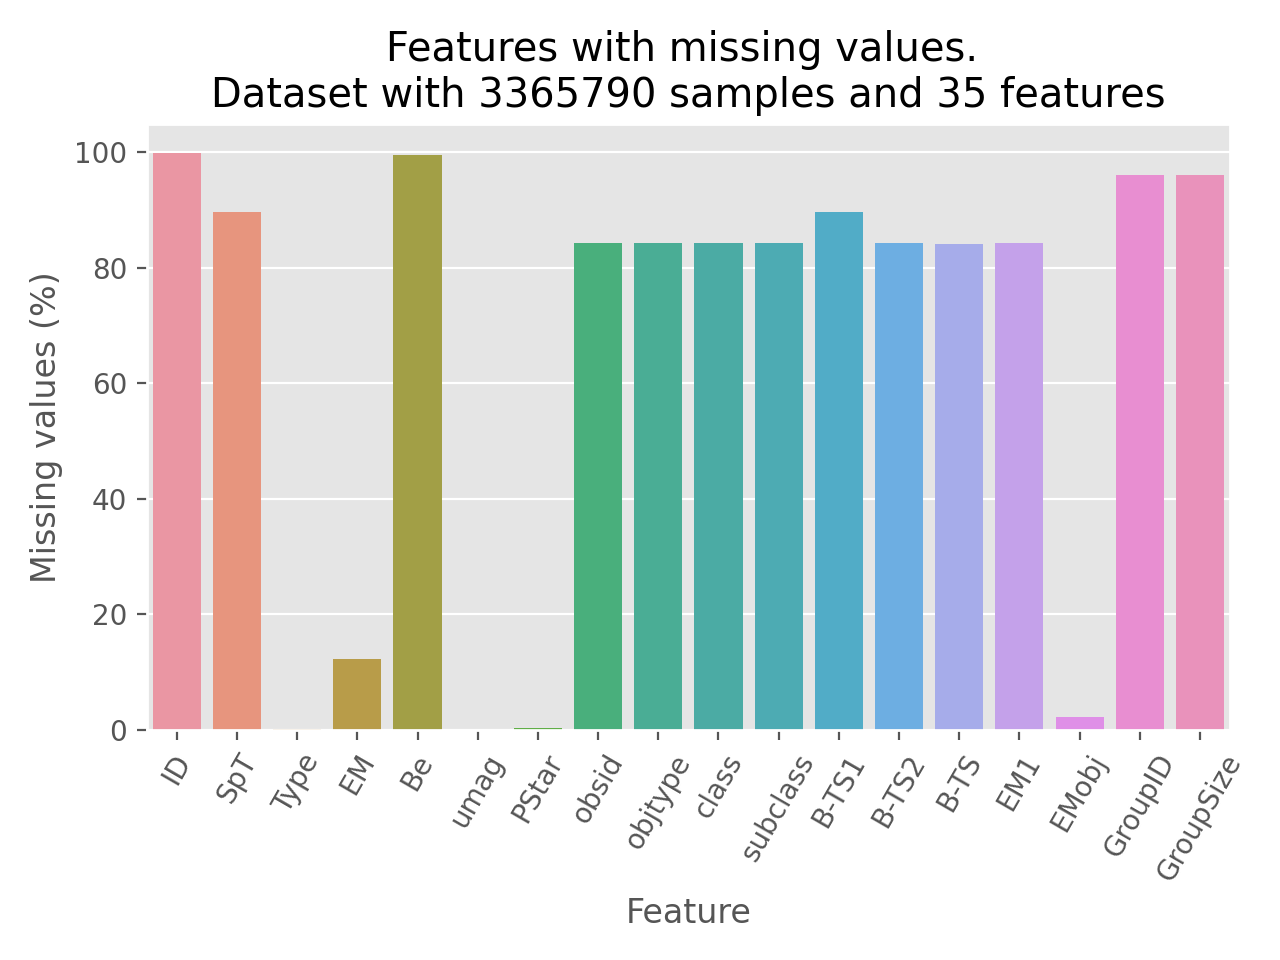
\includegraphics[width=1\linewidth]{plots/MissingValues/aidelman_missing.png}
    \label{fig:missing}
    \caption{Features with missing values}
\end{figure}

\begin{figure}
    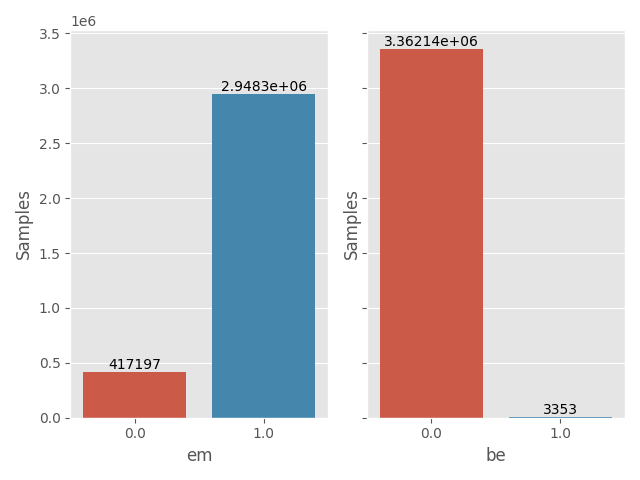
\includegraphics[width=0.49\linewidth]{plots/ClassFeaturesDistribution/aidelman_distribution.png}
    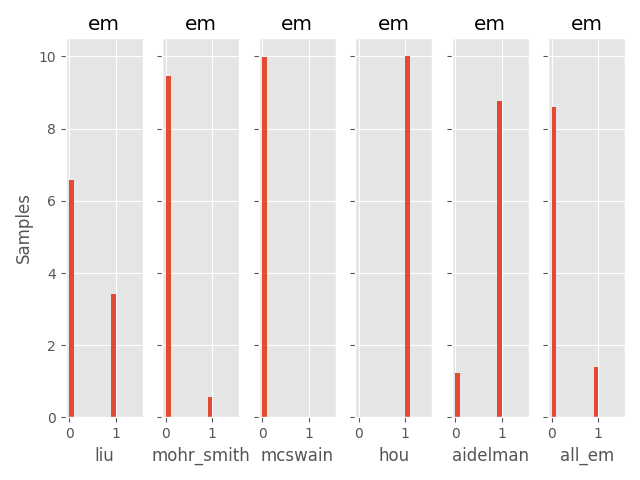
\includegraphics[width=0.49\linewidth]{plots/ClassDistributionComparison/histograms.png}
    \label{fig:aidelman_distribution}
    \caption{EM and Be class distribution for the UNLP-Stars dataset (left) and 
    comparison of EM class distribution between the new dataset and previous ones (right). This figure assumes missing values correspond to not EM and not Be classes.}
\end{figure}



\begin{figure}
    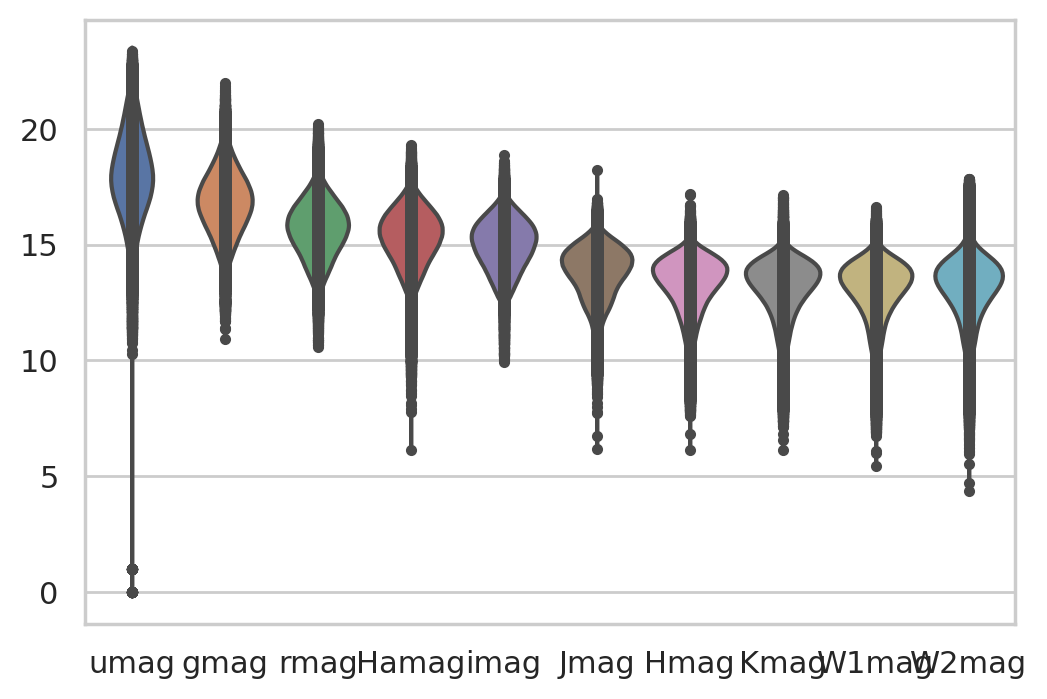
\includegraphics[width=0.49\linewidth]{plots/FeatureDistributions/aidelman_raw_violin.png}
    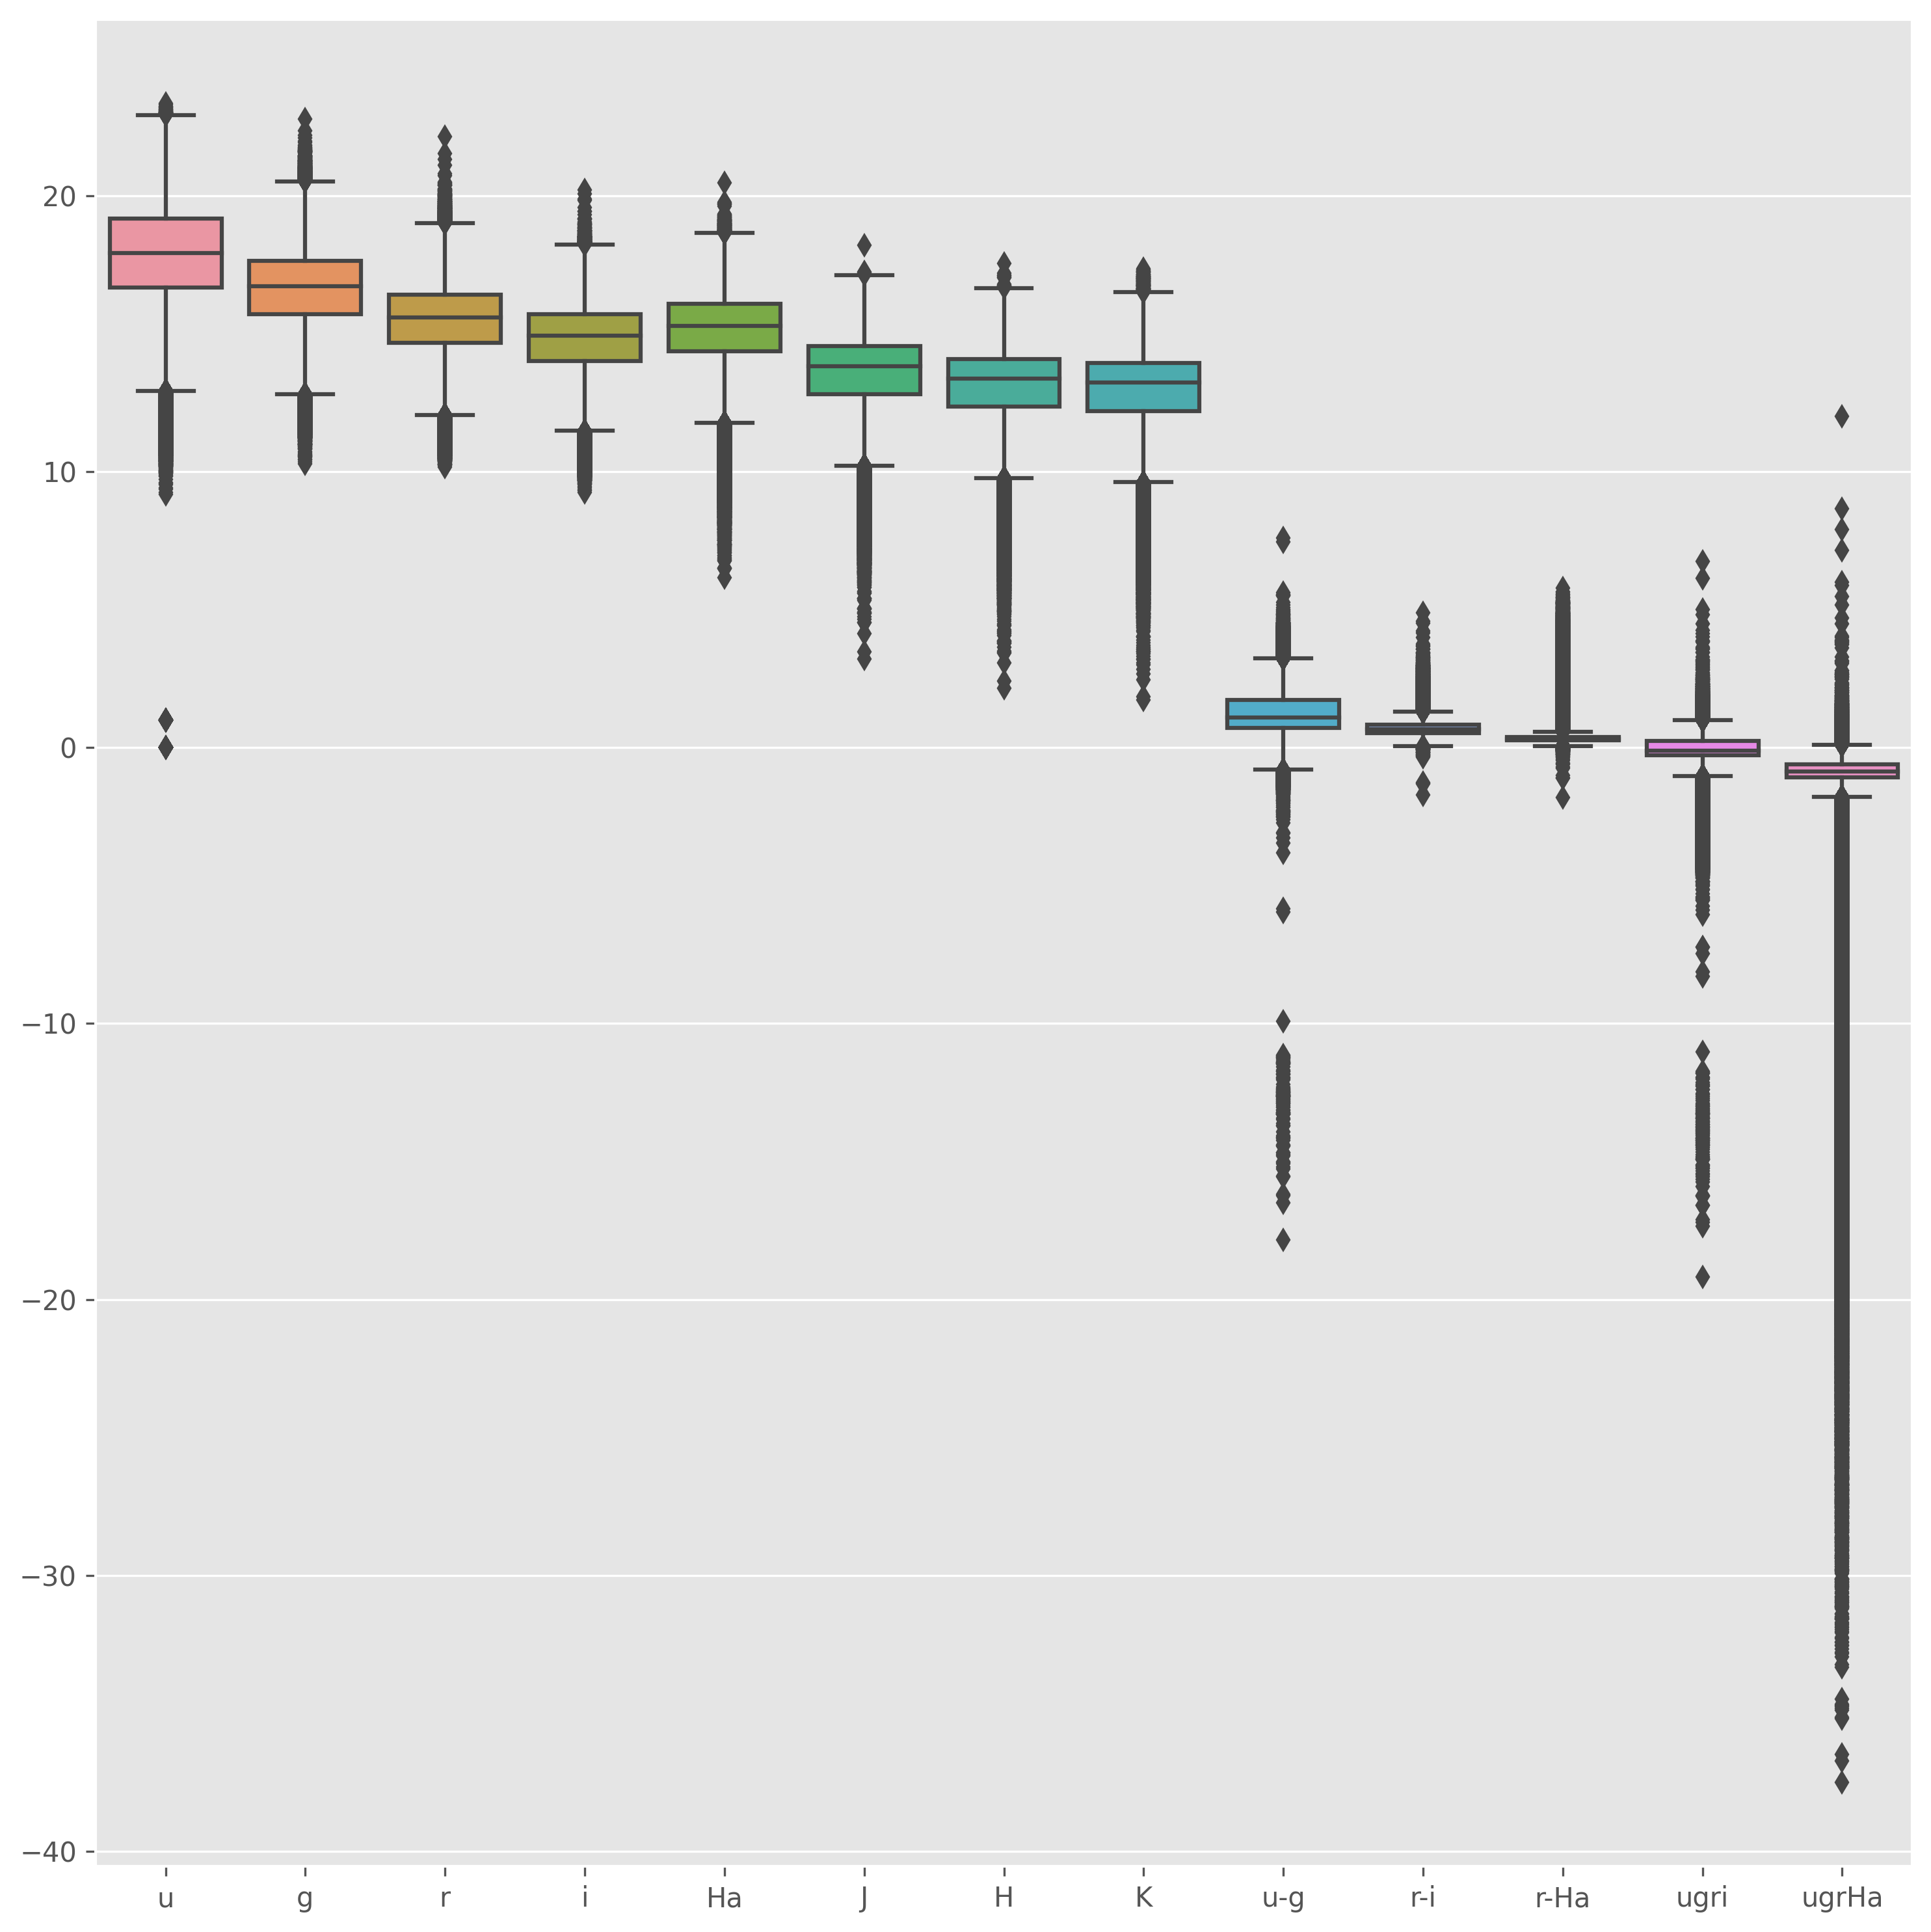
\includegraphics[width=0.49\linewidth]{plots/FeatureDistributions/aidelman_distribution.png}
    \label{fig:violin}
    \caption{Violin and box plot of features}
\end{figure}


\begin{figure}
    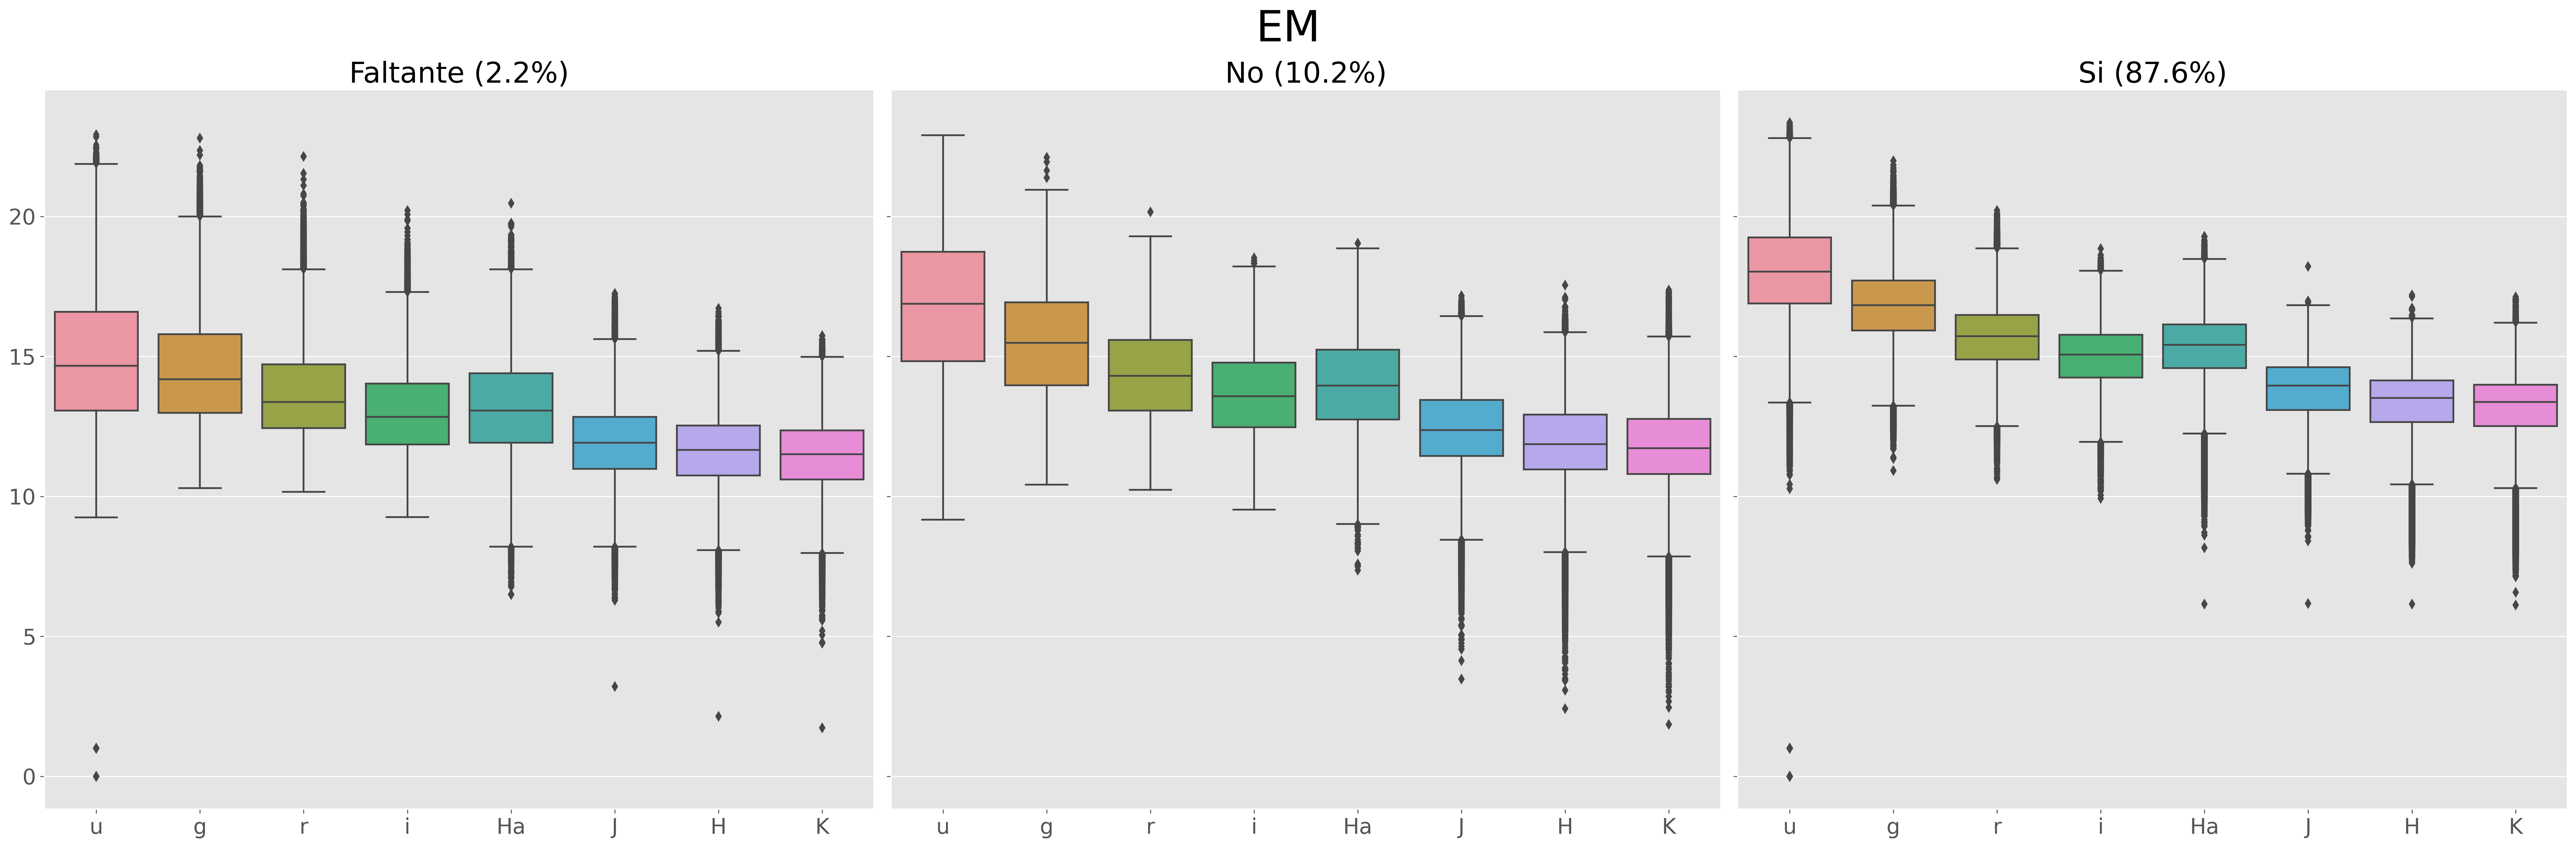
\includegraphics[width=1\linewidth]{plots/FeatureDistributions/aidelman_EM_mag.png}
    \label{fig:violin}
    \caption{Per-class boxplot for the EM feature}
\end{figure}


\begin{figure}
    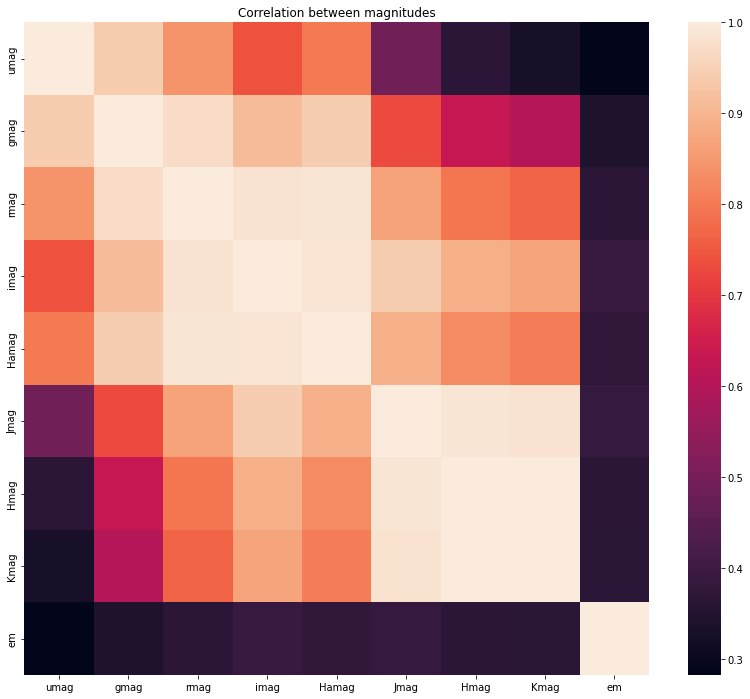
\includegraphics[width=0.3\linewidth]{plots/FeatureCorrelations/aidelman_raw.png}
    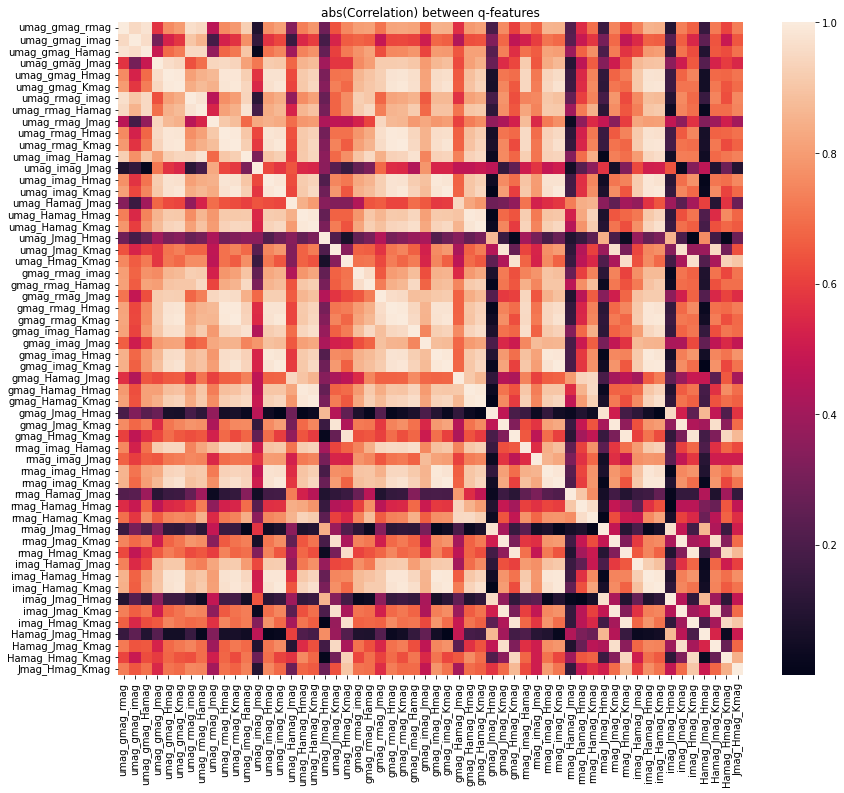
\includegraphics[width=0.3\linewidth]{plots/FeatureCorrelations/aidelman_q3.png}
    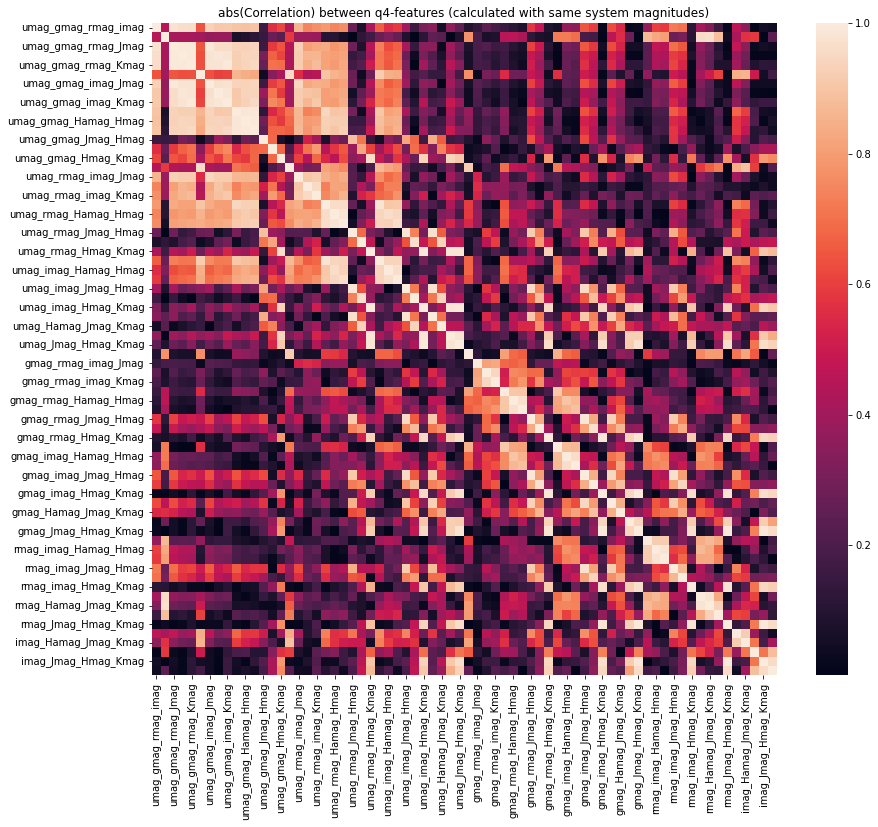
\includegraphics[width=0.3\linewidth]{plots/FeatureCorrelations/aidelman_q4.png}
    \label{fig:correlation}
    \caption{Correlation between raw, q3 and q4 features}
\end{figure}

\section{Experiments}

\subsection{EM classification}

\subsection{Baselines}
In order to establish a baseline performance for classifying EM objects, we split the dataset 80/20, obtaining training and test subsets, and we train three common models using SKLearn:

\begin{itemize}
    \item Random Forest, with a max depth of 6
    \item 3-layer neural network, with (10,10) hidden states
    \item Gradient Boosting, with 300 tree estimators
\end{itemize}

In all cases, the models could not overfit the training data even with a large capacity (ie, GB with 300 tree estimators). Furthermore, the class imbalance is biasing the model towards a greater recall (~99\%).

\begin{table}
\centering
\begin{tabular}[]{lccc}
    \toprule
     Model (Train) & f-score & precision & recall\\
    \midrule
    RandomForestClassifier &  0.951191 &  0.908095 & 0.998581\\
    MLPClassifier & 0.954169  & 0.919153 & 0.991958\\
    GradientBoostingClassifier  & 0.951439 &  0.911145 & 0.995461\\
    \midrule
     Model (Test) & f-score  & precision  &   recall\\
    \midrule
    RandomForestClassifier &  0.951387 &  0.908369 & 0.998682\\
    MLPClassifier & 0.954212 & 0.919330 & 0.991846\\
    GradientBoostingClassifier & 0.951507 &  0.911367 & 0.995345\\
    \bottomrule
\end{tabular}    
\end{table}


\subsubsection{Classification via Neural Networks}

Given that the baseline models could not fit the training dataset, we evaluated three deep neural network models, trained with the ADAM optimizer for 500 epochs. The networks consist of Dense layers with the following three topologies:

\begin{enumerate}
    \item Small: Neurons per layer: 64,32,16,8 
    \item Medium: Neurons per layer: 256,128,64,32,16
    \item Large: Neurons per layer: 1024,512,256,64,32
\end{enumerate}


Additionally, we evaluate using as input $q3$ and $q4$ features vs the $raw$ features (rmag, umag, etc). We employ class weights to achieve a better balance between precision and recall. We also train models to classify stars in as Be or not.

The results for the EM class (figure  \ref{fig:aidelman_em}) show that the $raw$ features consistently achieve slighty better results (1\%) than $q3$ or $q4$. Additionally, all models achieve very similar results, but the simplest model is in general slightly better (1\%) than the more complex ones.

The results for the Be task (figure \ref{fig:aidelman_be}) are much worse, achieving a very small precision. This is caused by the low number of samples labelled as Be.

\begin{figure}
    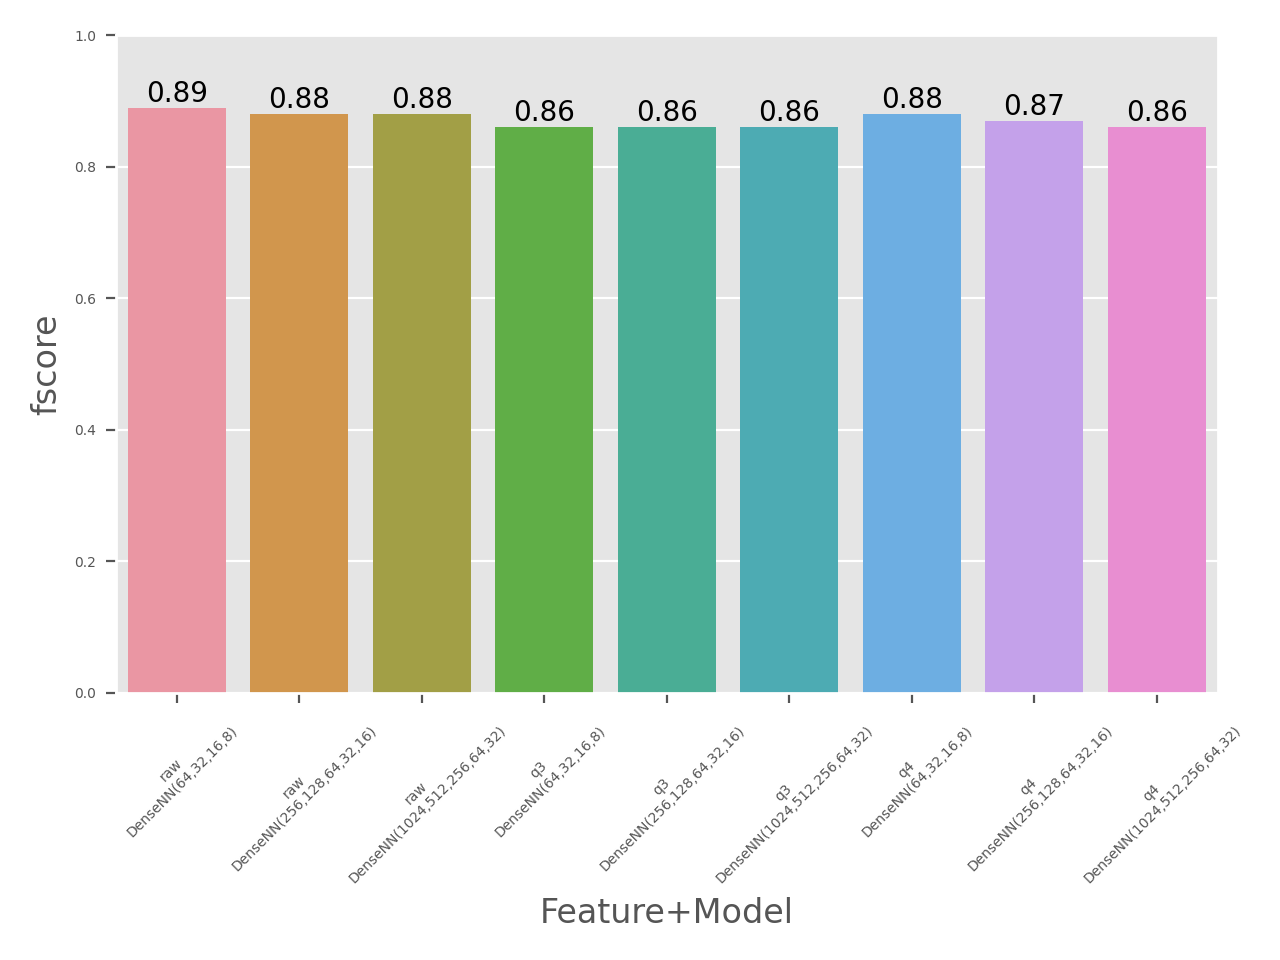
\includegraphics[width=0.49\linewidth]{plots/EvaluateClassifiers/aidelman_em_train_fscore.png}
    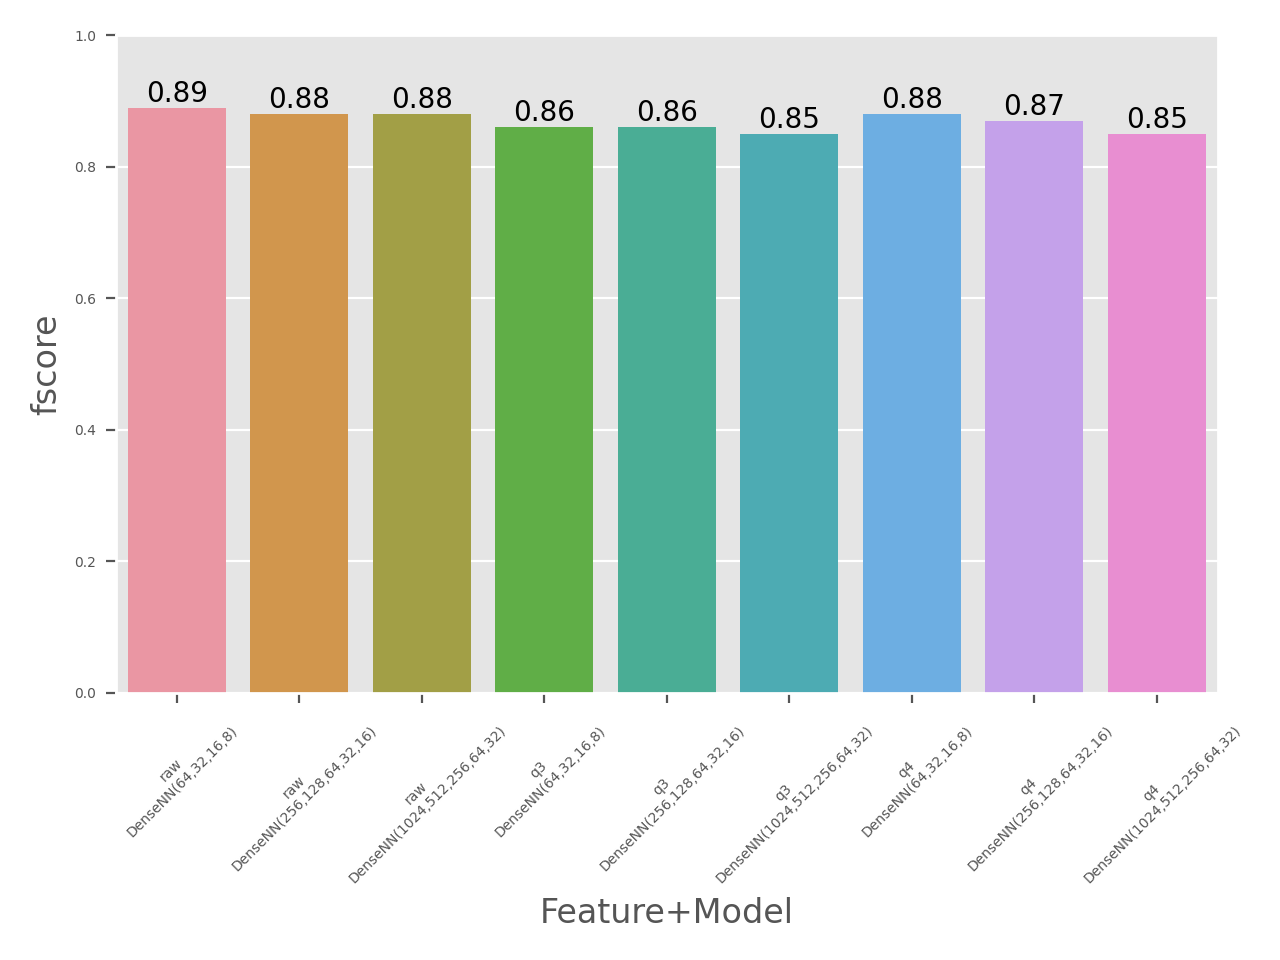
\includegraphics[width=0.49\linewidth]{plots/EvaluateClassifiers/aidelman_em_test_fscore.png}\\
    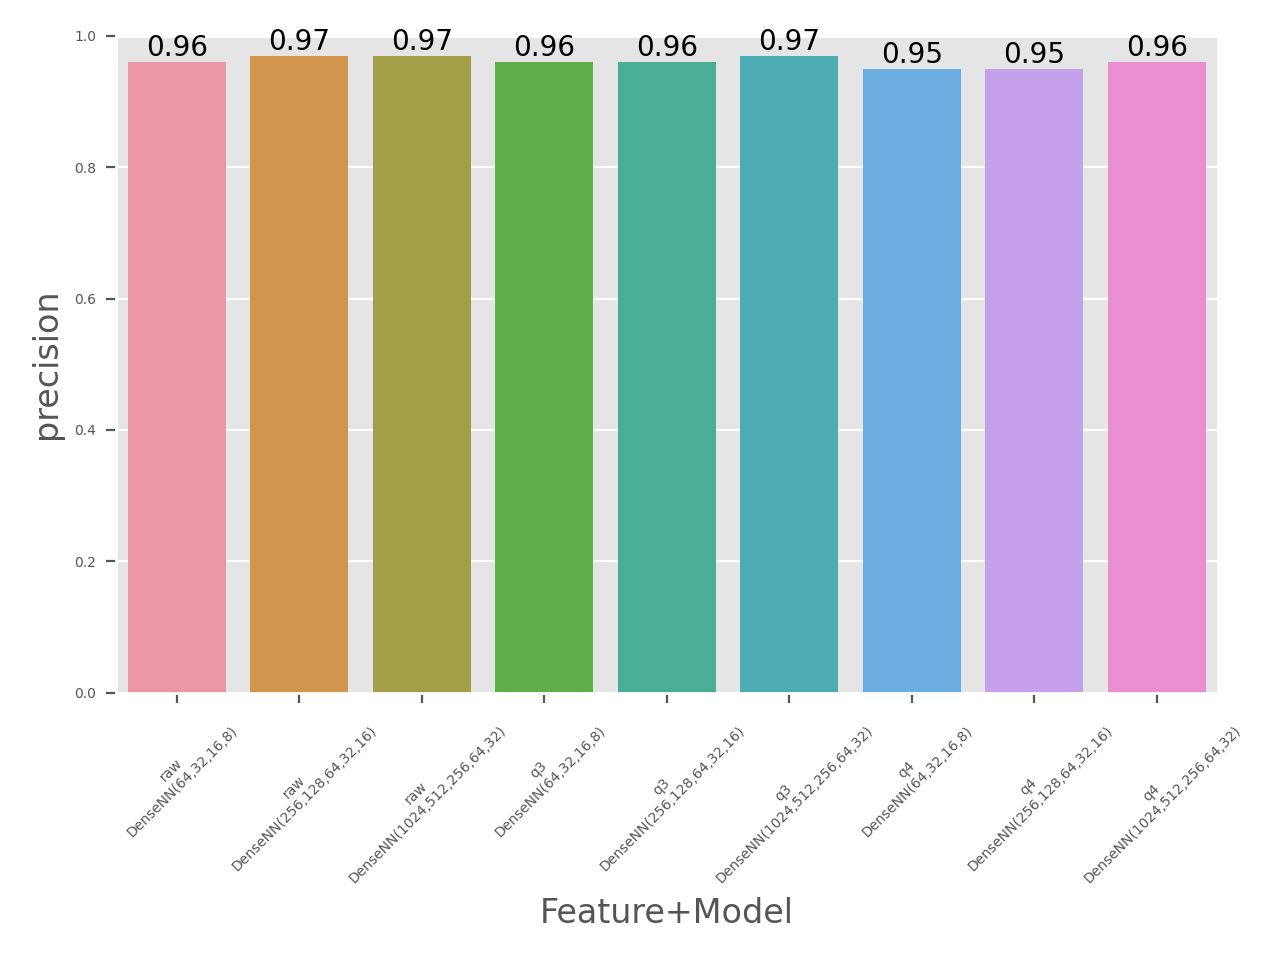
\includegraphics[width=0.49\linewidth]{plots/EvaluateClassifiers/aidelman_em_train_precision.png}
    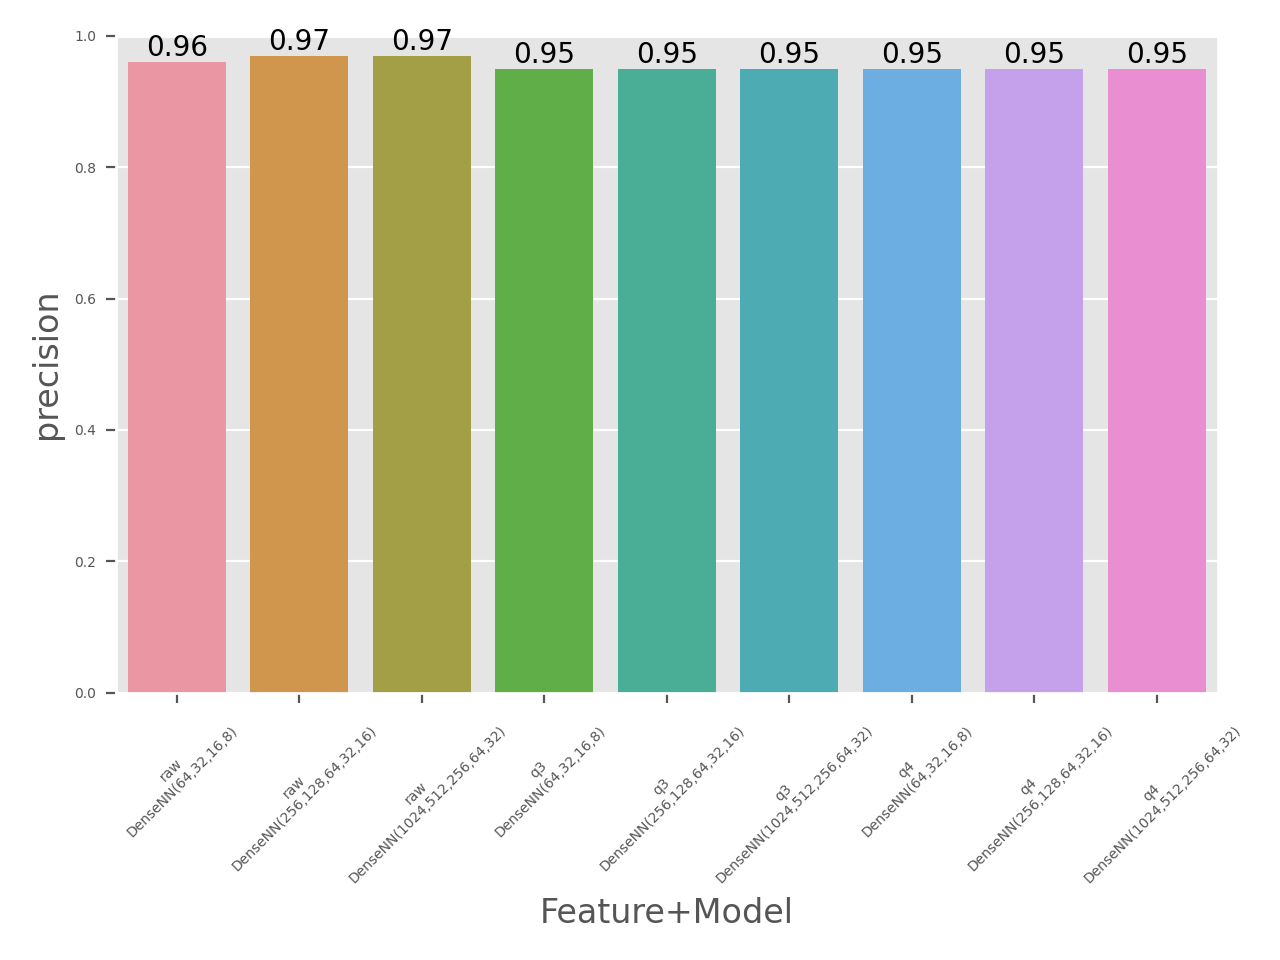
\includegraphics[width=0.49\linewidth]{plots/EvaluateClassifiers/aidelman_em_test_precision.png}\\
    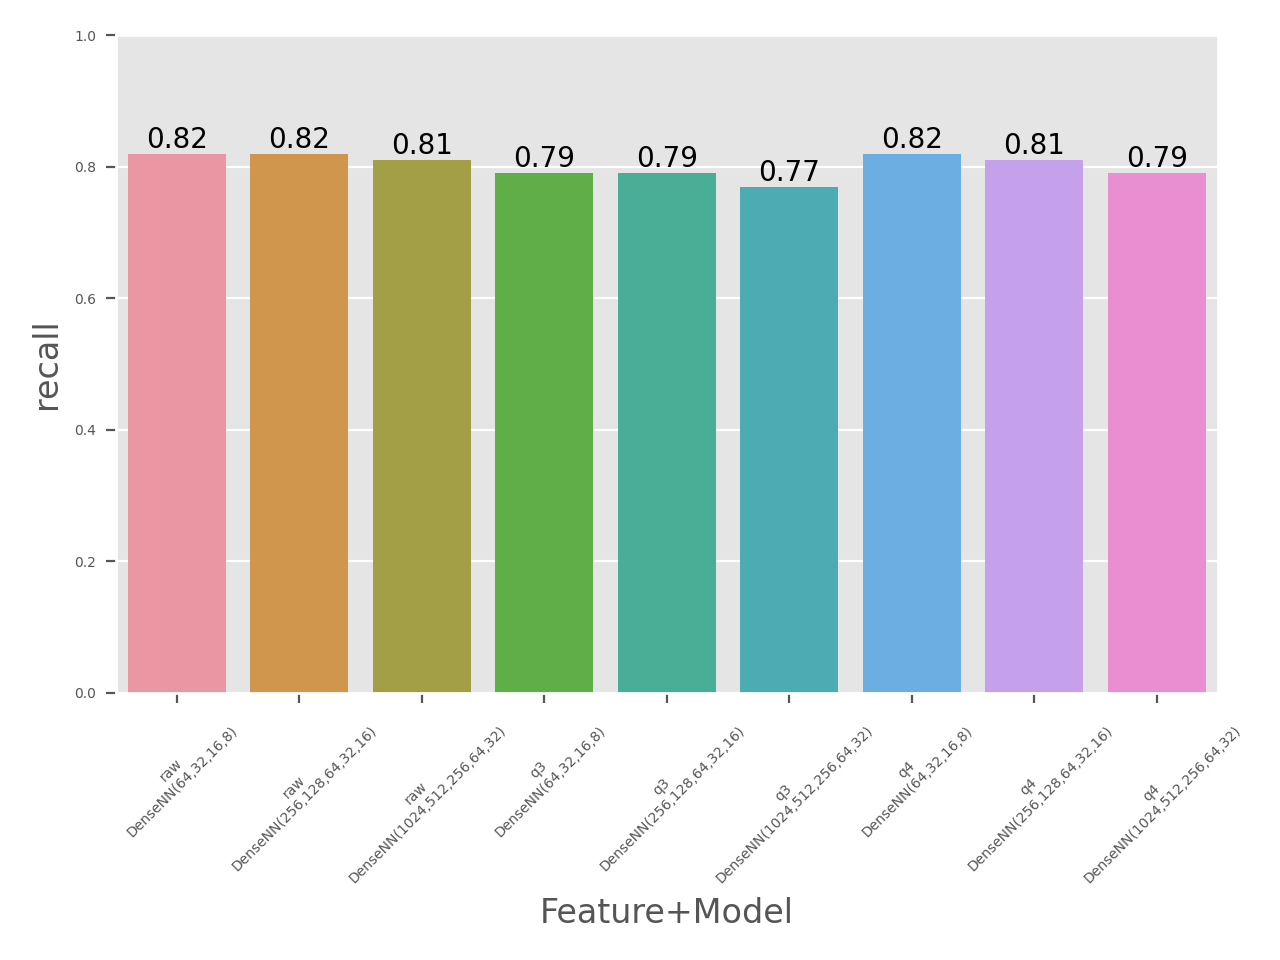
\includegraphics[width=0.49\linewidth]{plots/EvaluateClassifiers/aidelman_em_train_recall.png}
    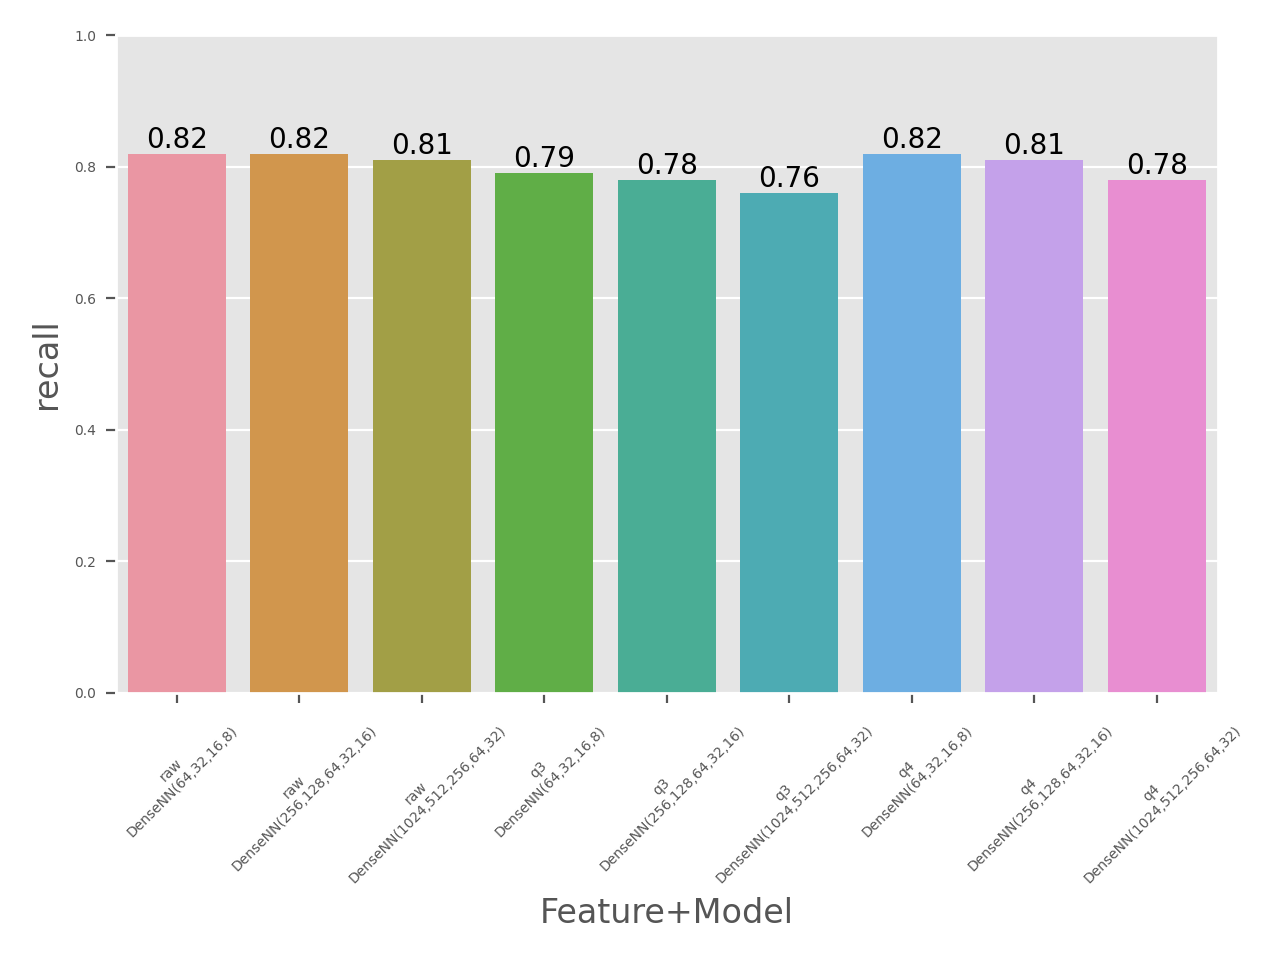
\includegraphics[width=0.49\linewidth]{plots/EvaluateClassifiers/aidelman_em_test_recall.png}\\
    \label{fig:aidelman_em}
    \caption{F-Score for train (left) and test (right) sets when classifying stars as EM or not (row 1); row 2 and 3 correspond to precision and recall.}
\end{figure}


\begin{figure}
    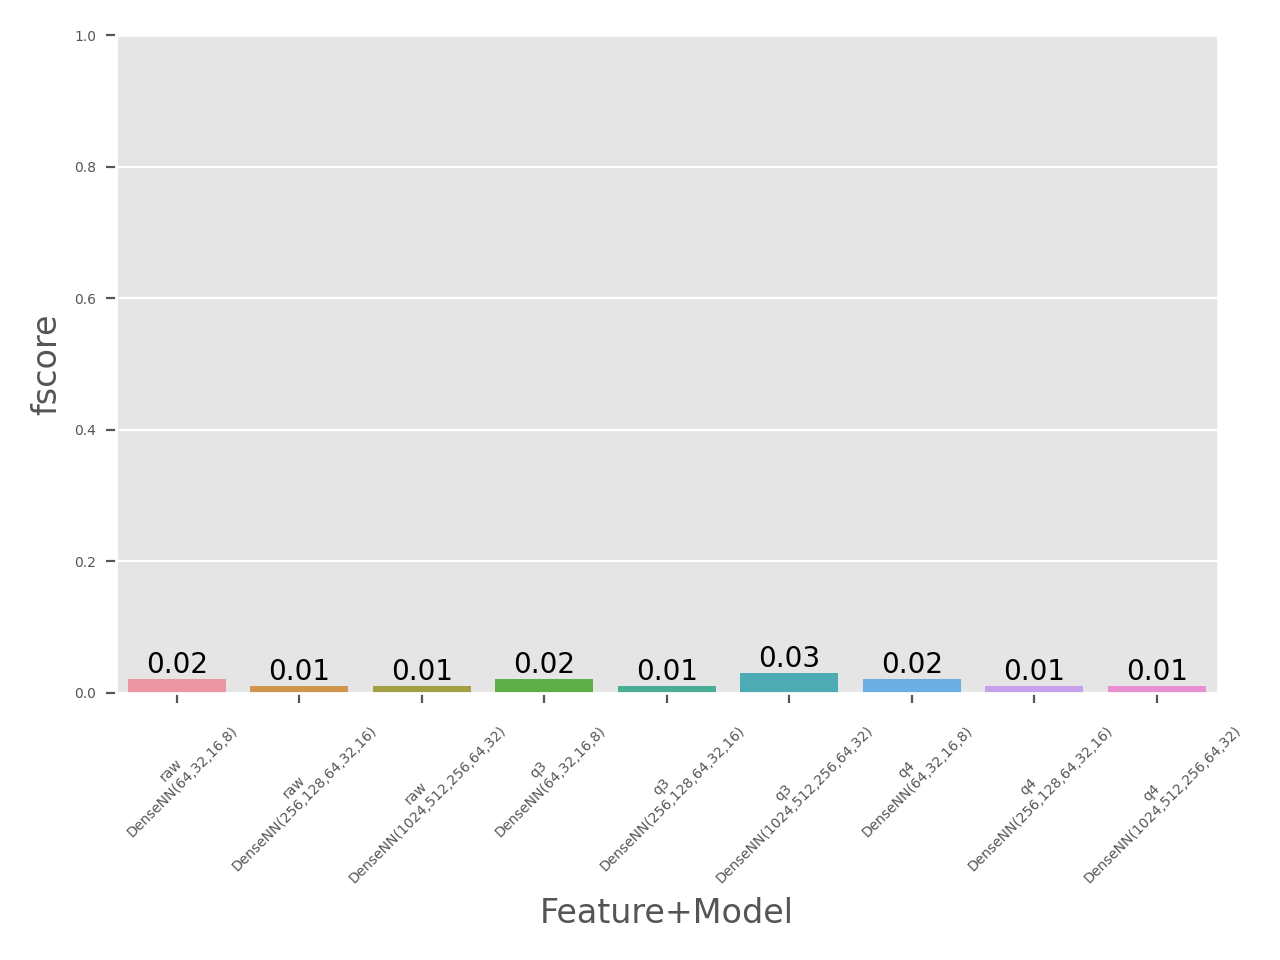
\includegraphics[width=0.49\linewidth]{plots/EvaluateClassifiers/aidelman_be_train_fscore.png}
    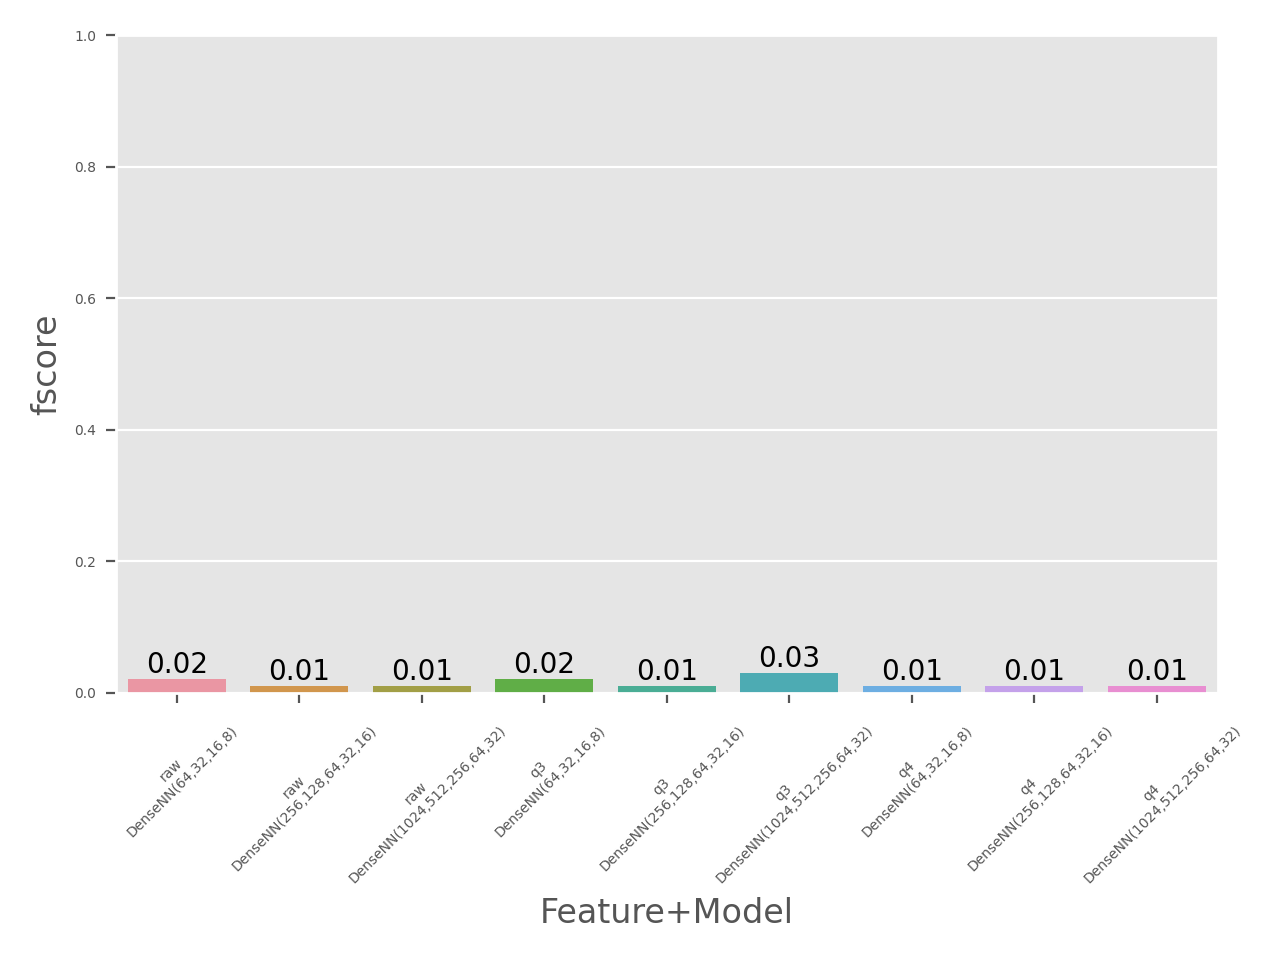
\includegraphics[width=0.49\linewidth]{plots/EvaluateClassifiers/aidelman_be_test_fscore.png}\\
    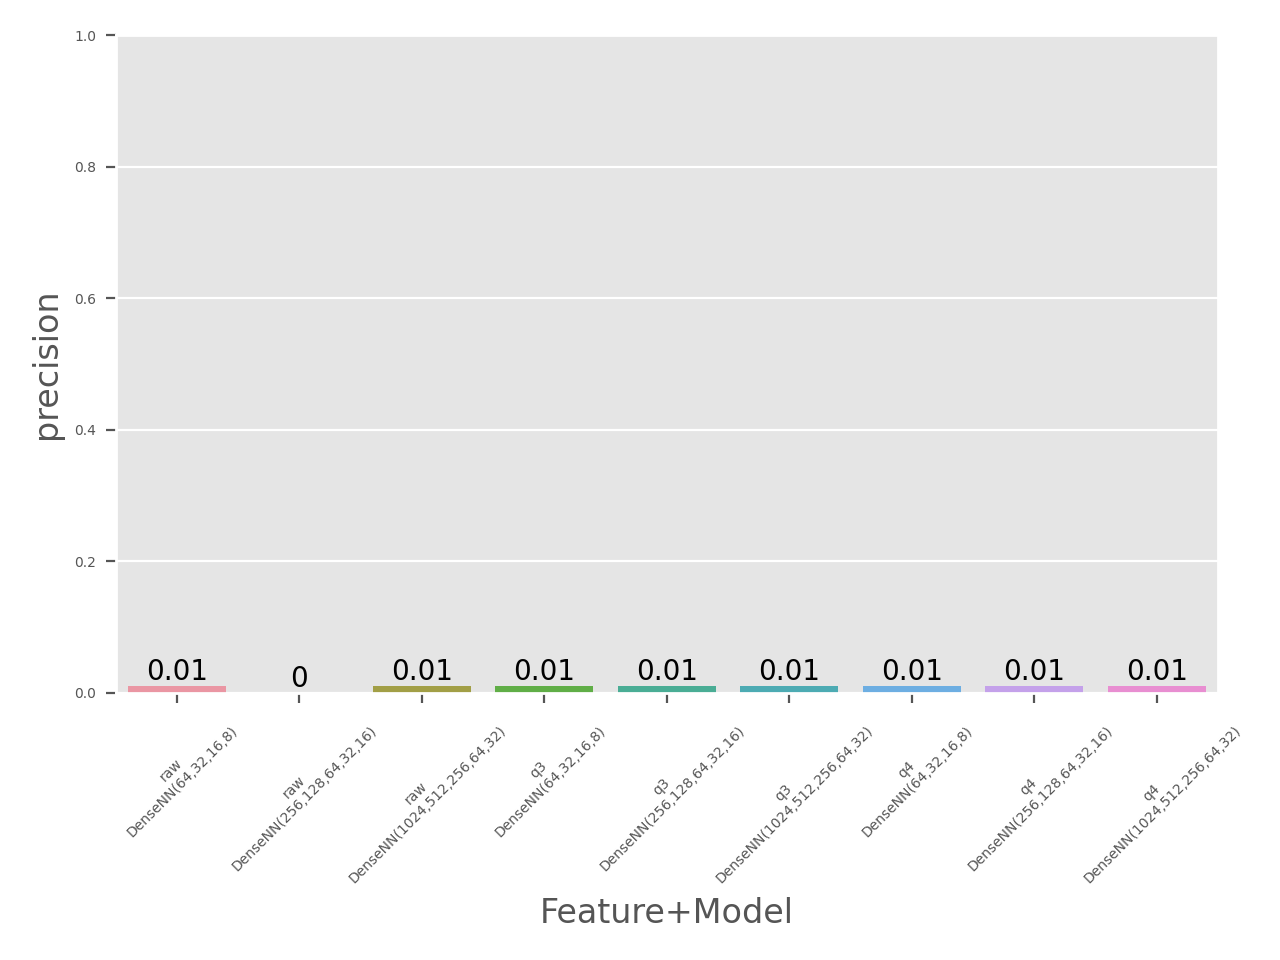
\includegraphics[width=0.49\linewidth]{plots/EvaluateClassifiers/aidelman_be_train_precision.png}
    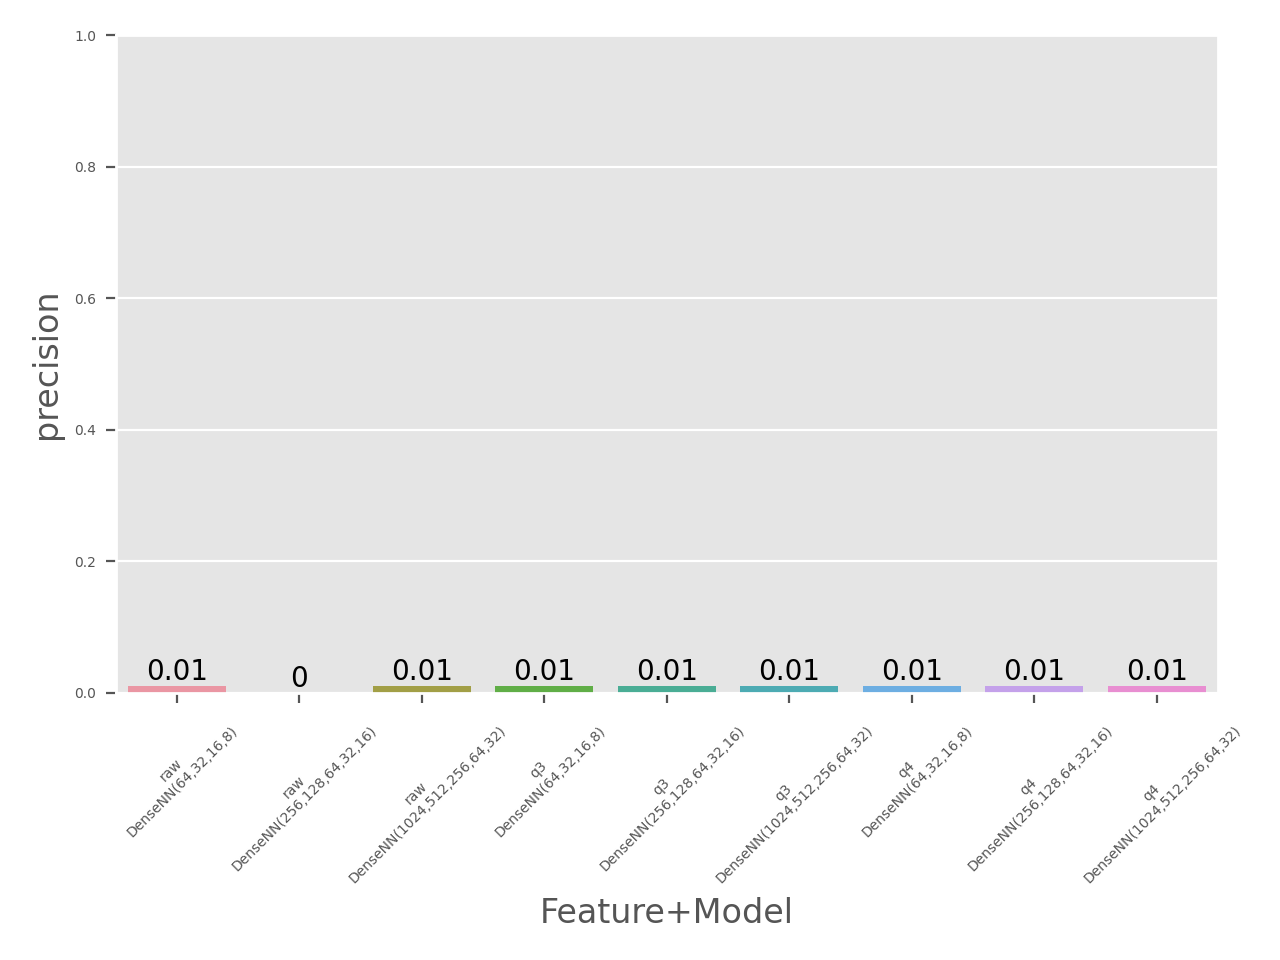
\includegraphics[width=0.49\linewidth]{plots/EvaluateClassifiers/aidelman_be_test_precision.png}\\
    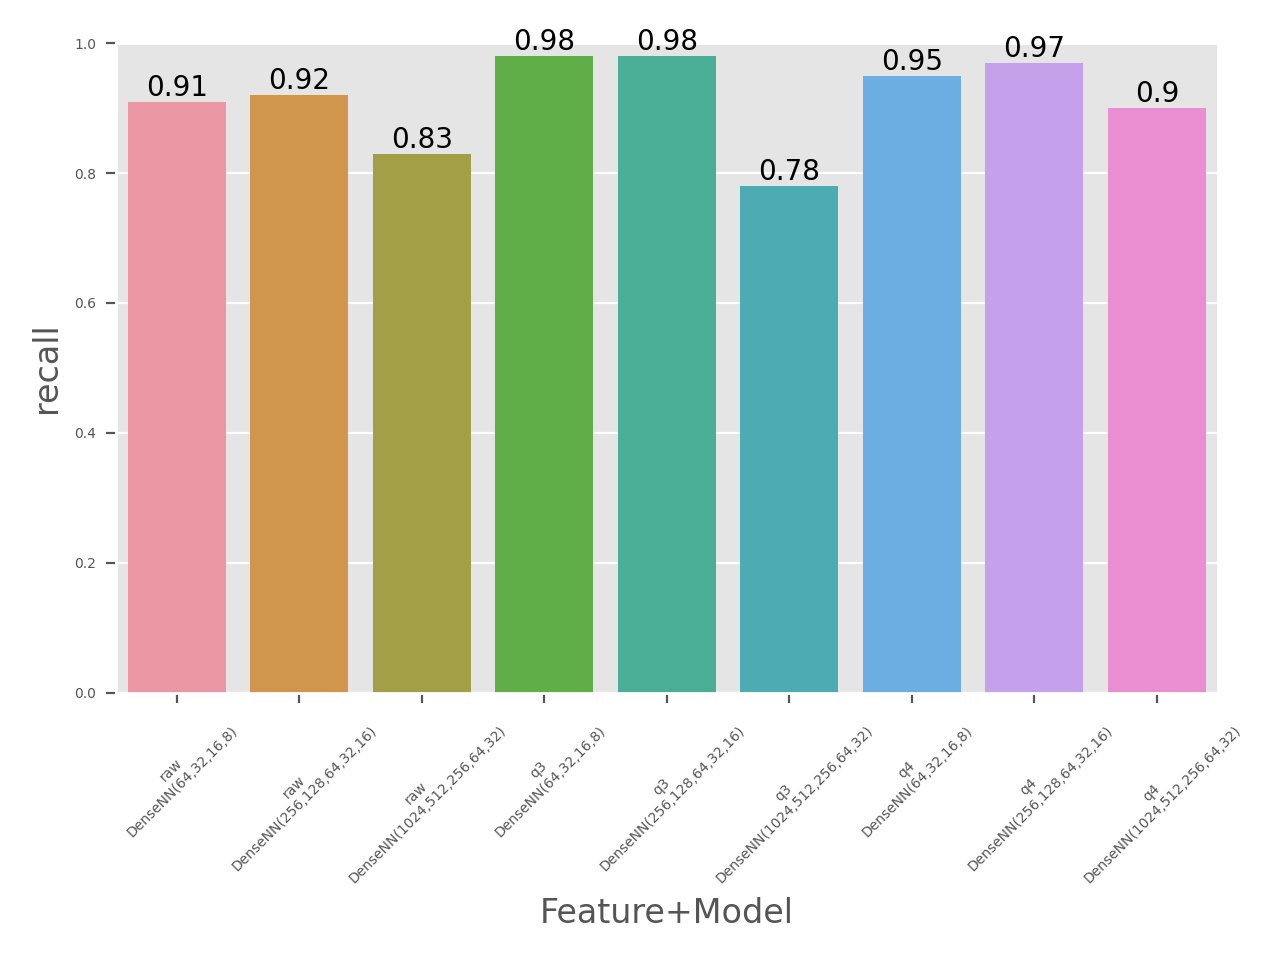
\includegraphics[width=0.49\linewidth]{plots/EvaluateClassifiers/aidelman_be_train_recall.png}
    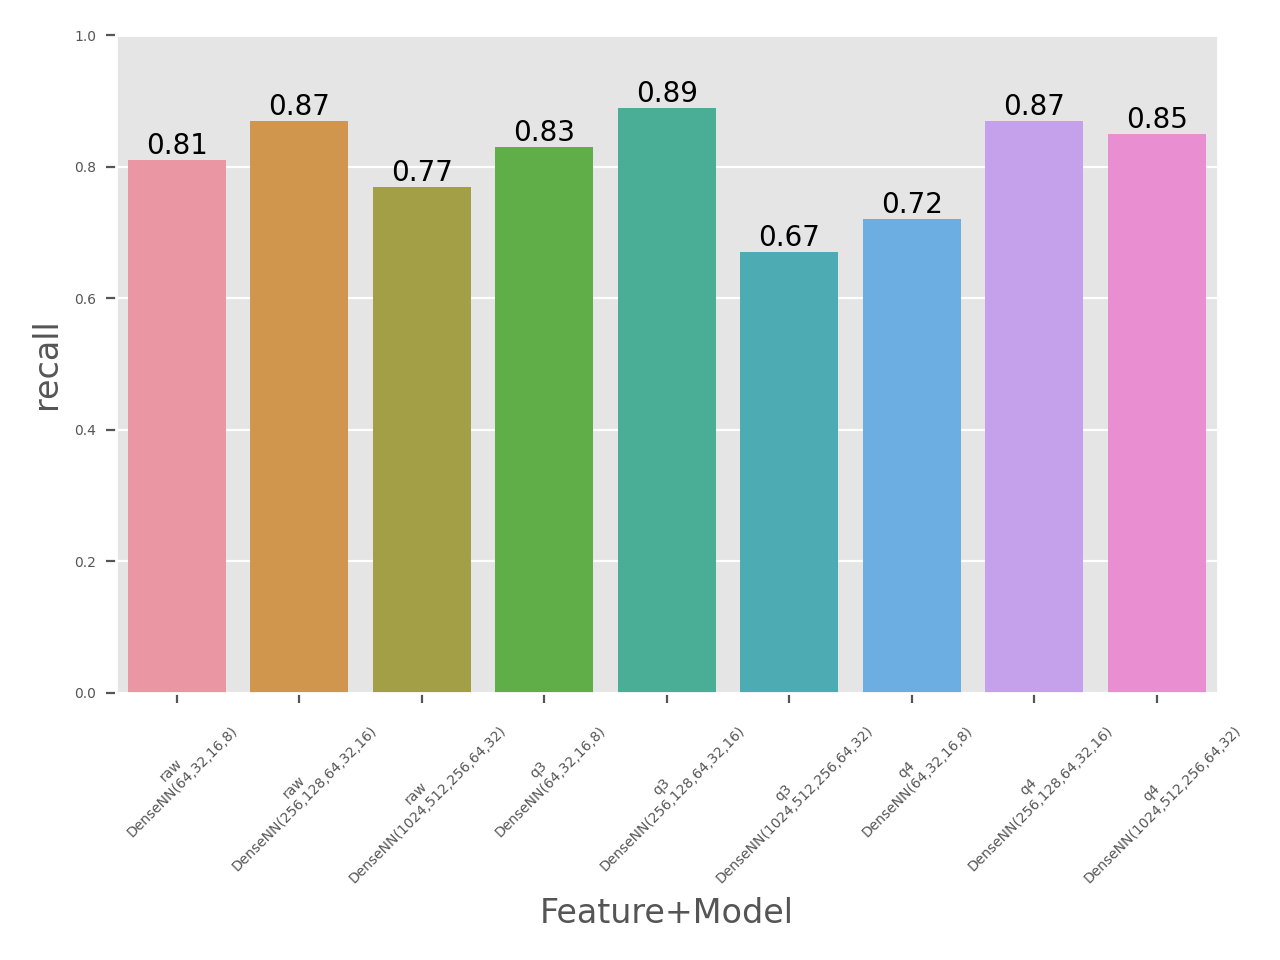
\includegraphics[width=0.49\linewidth]{plots/EvaluateClassifiers/aidelman_be_test_recall.png}\\
    \label{fig:aidelman_be}
    \caption{F-Score for train (left) and test (right) sets when classifying stars as Be or not (row 1); row 2 and 3 correspond to precision and recall.}
\end{figure}

\subsubsection{Analysis of training set size dependence}

Since even deep neural network models cannot overfit the training data, we investigated the effect of the training set size on the model's performance. Given that smaller training sets should be easier to overfit, we would expect the test scores to worsen while the training scores improve if we reduce the training set size. However, from our experiments even when training with 10\% of the total dataset (~300.000 samples), the training and test metrics show no significant different with respect to using 90\% of the dataset for training. This holds for all three neural network models and features.

\begin{figure}
        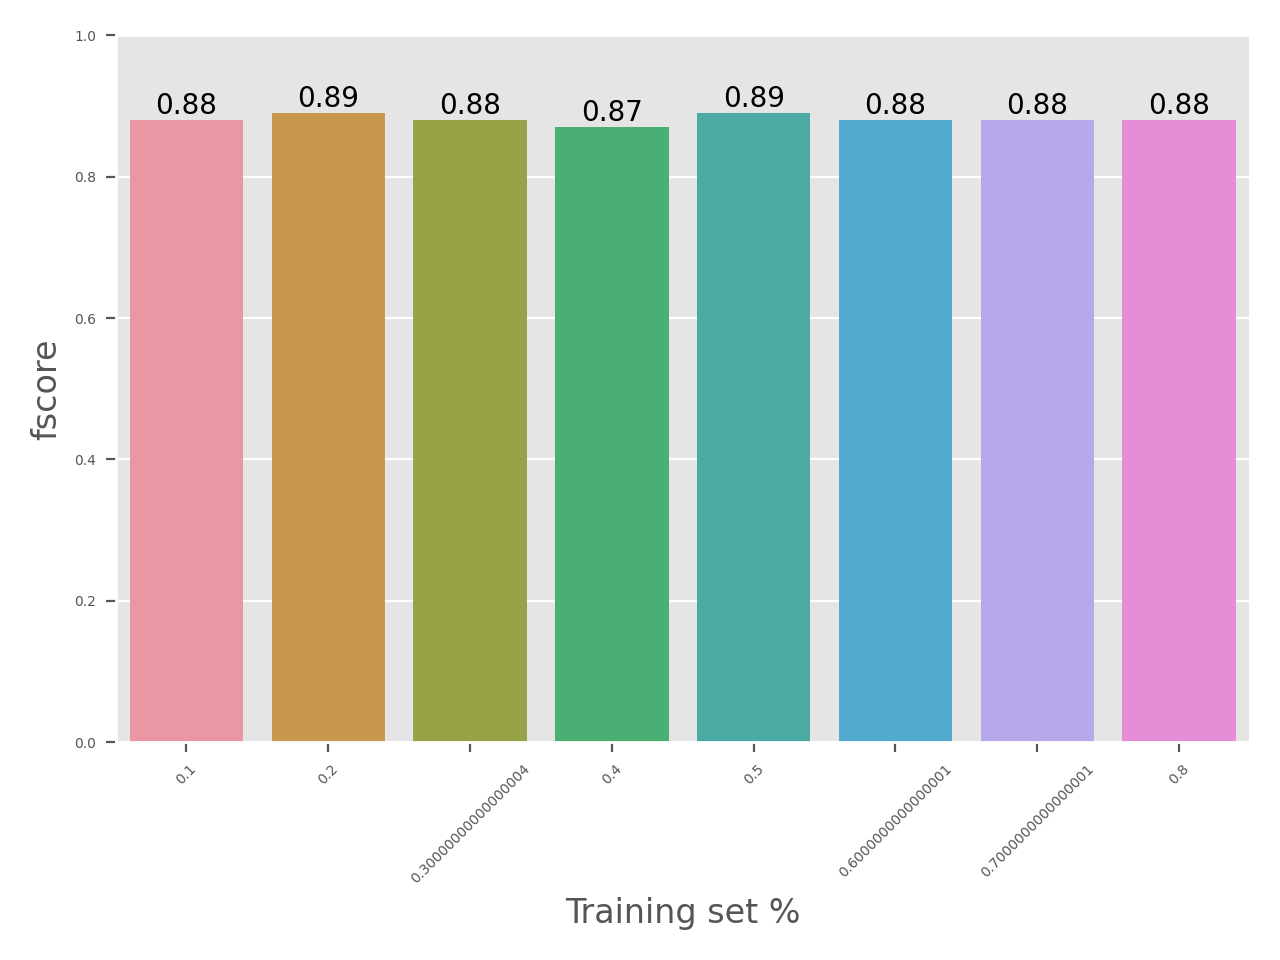
\includegraphics[width=0.49\linewidth]{plots/DetermineMinimumTrainingSet/aidelman_DenseNN(256,128,64,32,16)_em_raw_train_fscore.png}
        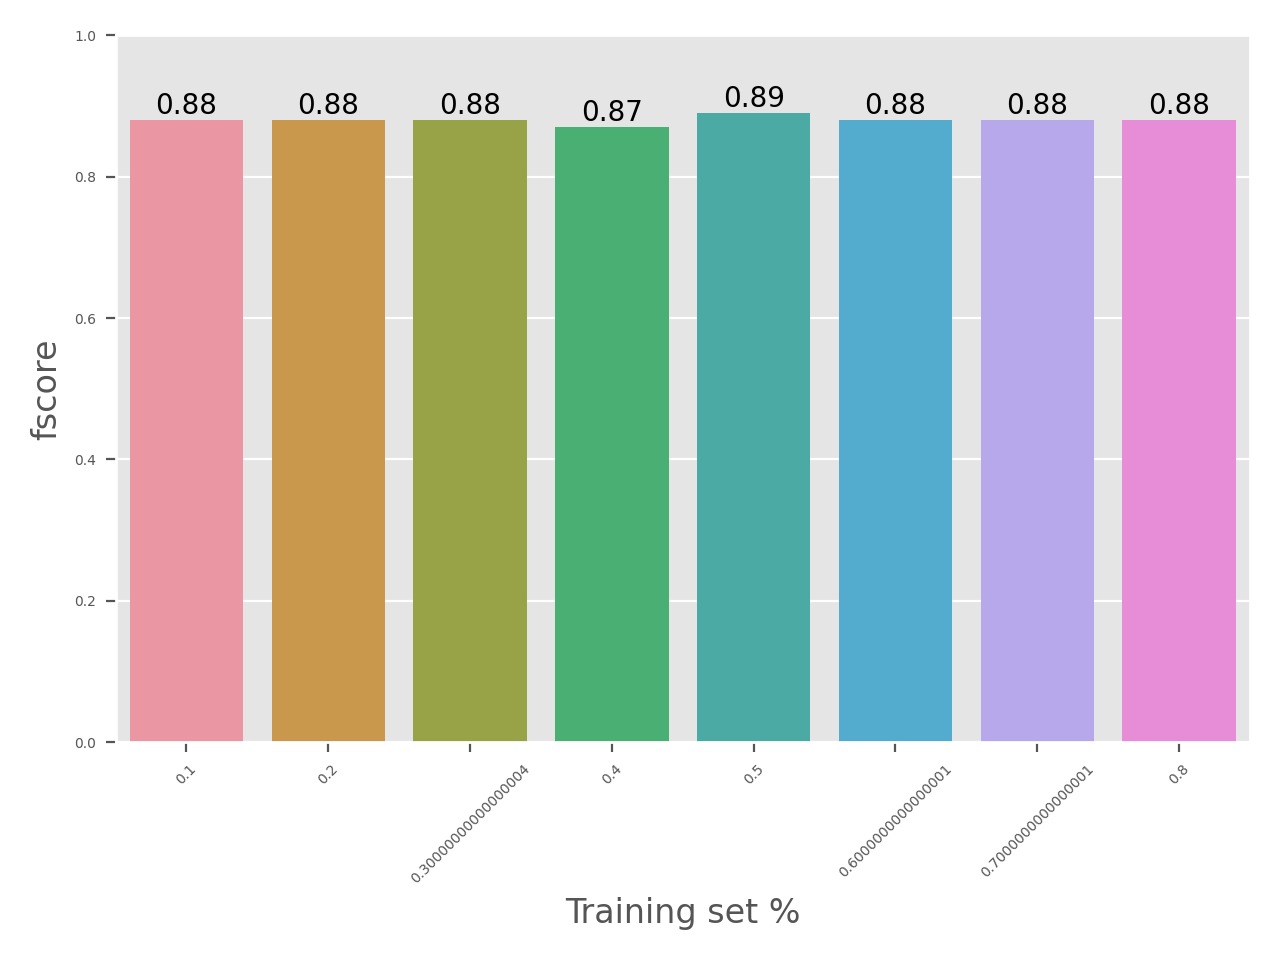
\includegraphics[width=0.49\linewidth]{plots/DetermineMinimumTrainingSet/aidelman_DenseNN(256,128,64,32,16)_em_raw_test_fscore.png}
        \caption{F-Score for train (left) and test (right) sets when classifying stars as EM or not, for various training set sizes (in percentage). Results for the $q3$ and $q4$ features and other neural network architectures are very similar.}
\end{figure}



\begin{figure}
    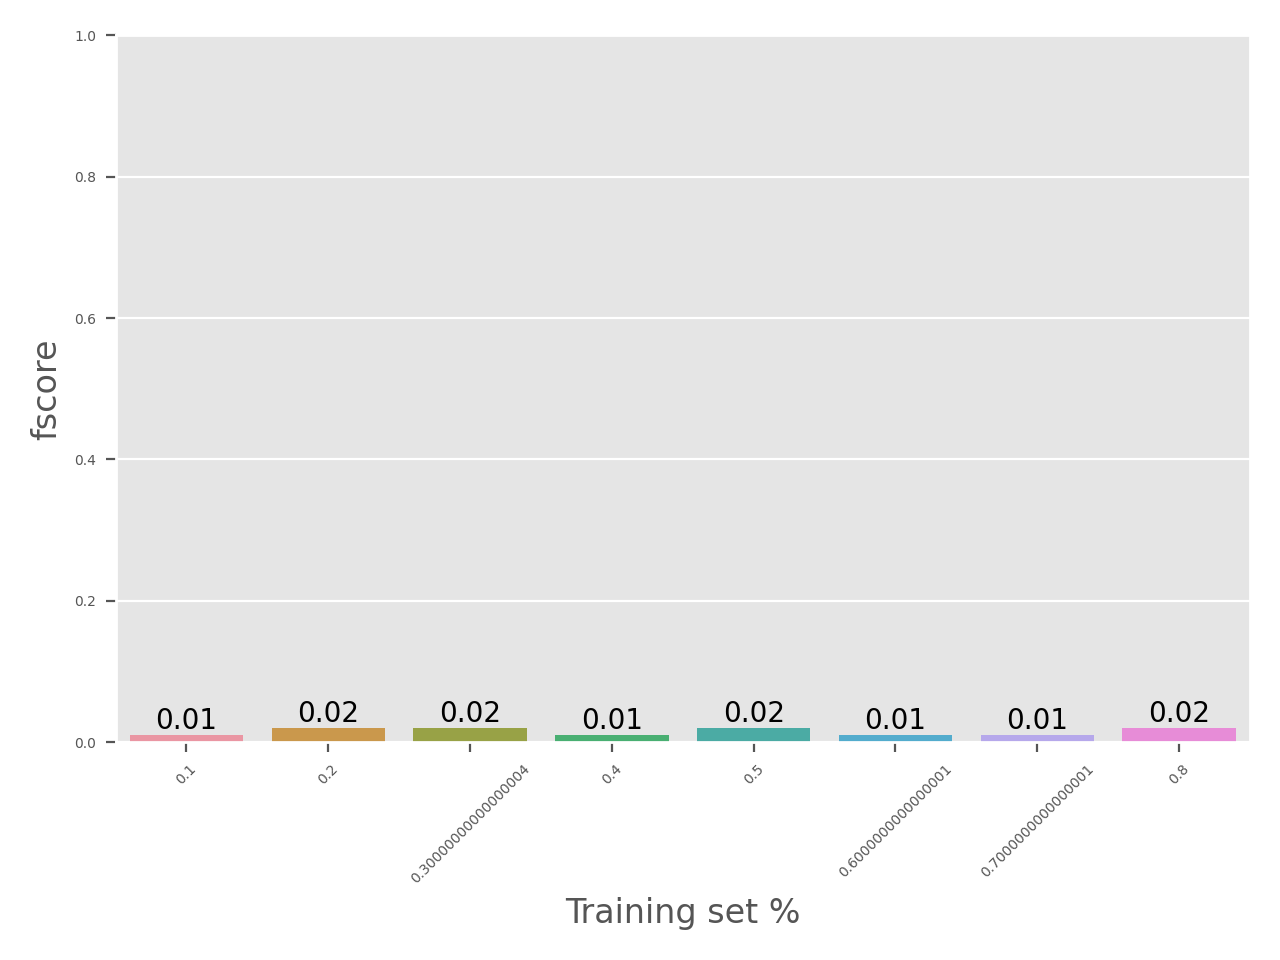
\includegraphics[width=0.49\linewidth]{plots/DetermineMinimumTrainingSet/aidelman_DenseNN(256,128,64,32,16)_be_raw_train_fscore.png}
    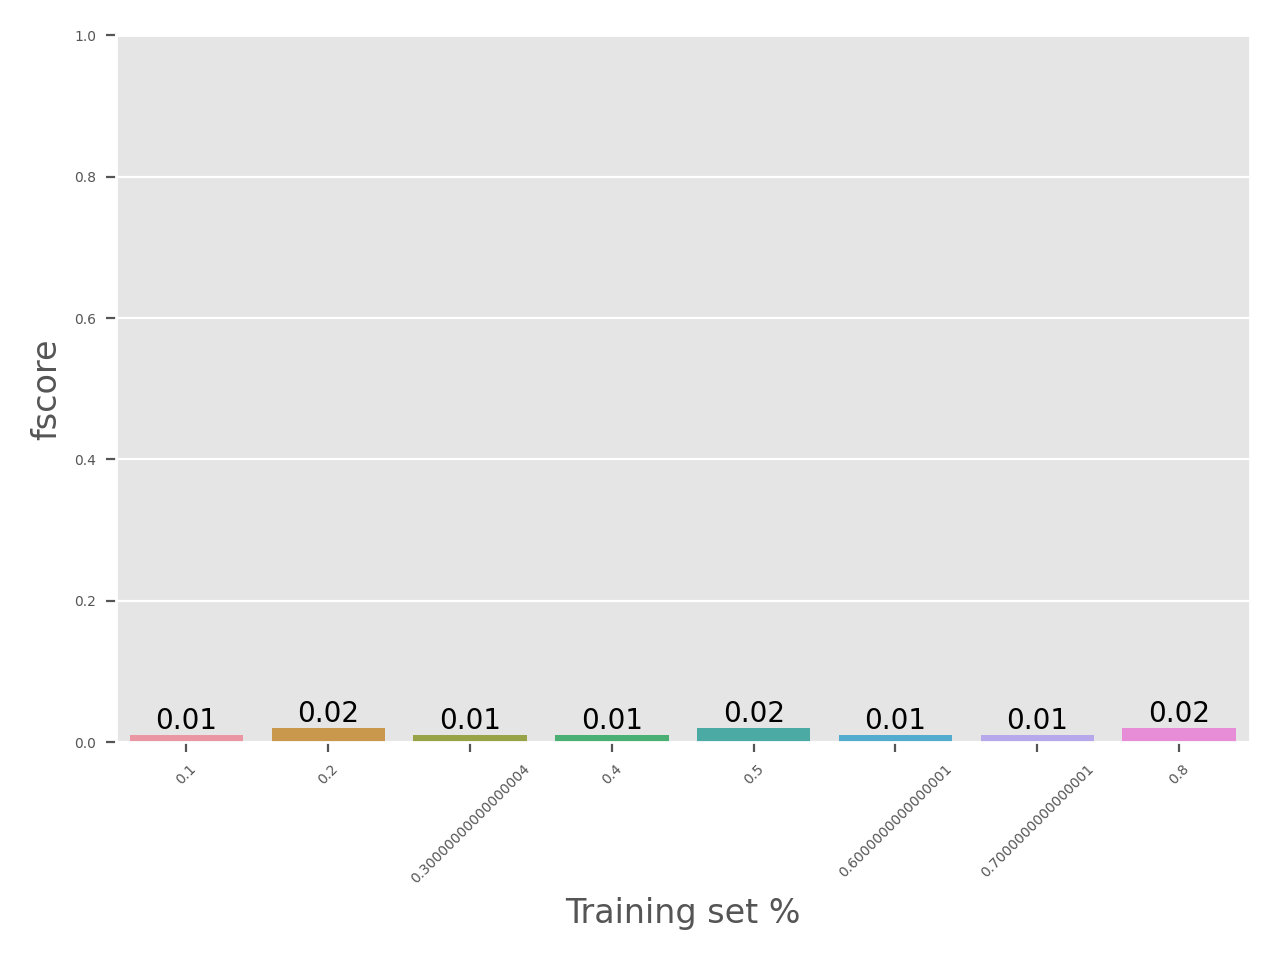
\includegraphics[width=0.49\linewidth]{plots/DetermineMinimumTrainingSet/aidelman_DenseNN(256,128,64,32,16)_be_raw_test_fscore.png}
    \caption{F-Score for train (left) and test (right) sets when classifying stars as Be or not, for various training set sizes (in percentage). Results for the $q3$ and $q4$ features and other neural network architectures are very similar.}
\end{figure}

% \begin{figure}
%     \includegraphics[width=0.49\linewidth]{plots/EvaluateClassifiers/aidelman_be_raw_train_fscore.png}
%     \includegraphics[width=0.49\linewidth]{plots/EvaluateClassifiers/aidelman_be_raw_test_fscore.png}
%     \caption{F-Score for train (left) and test (right) sets when classifying stars as BE or not.}
% \end{figure}

\end{document}